\documentclass[border=10pt]{standalone}

\usepackage{tikz}
\usepackage{tikzsymbols}
\usetikzlibrary{calc,patterns,shapes.geometric}

\def\centerarc[#1](#2)(#3:#4:#5){\draw[#1] ($(#2)+({#5*cos(#3)},{#5*sin(#3)})$) arc (#3:#4:#5);}

\begin{document}
	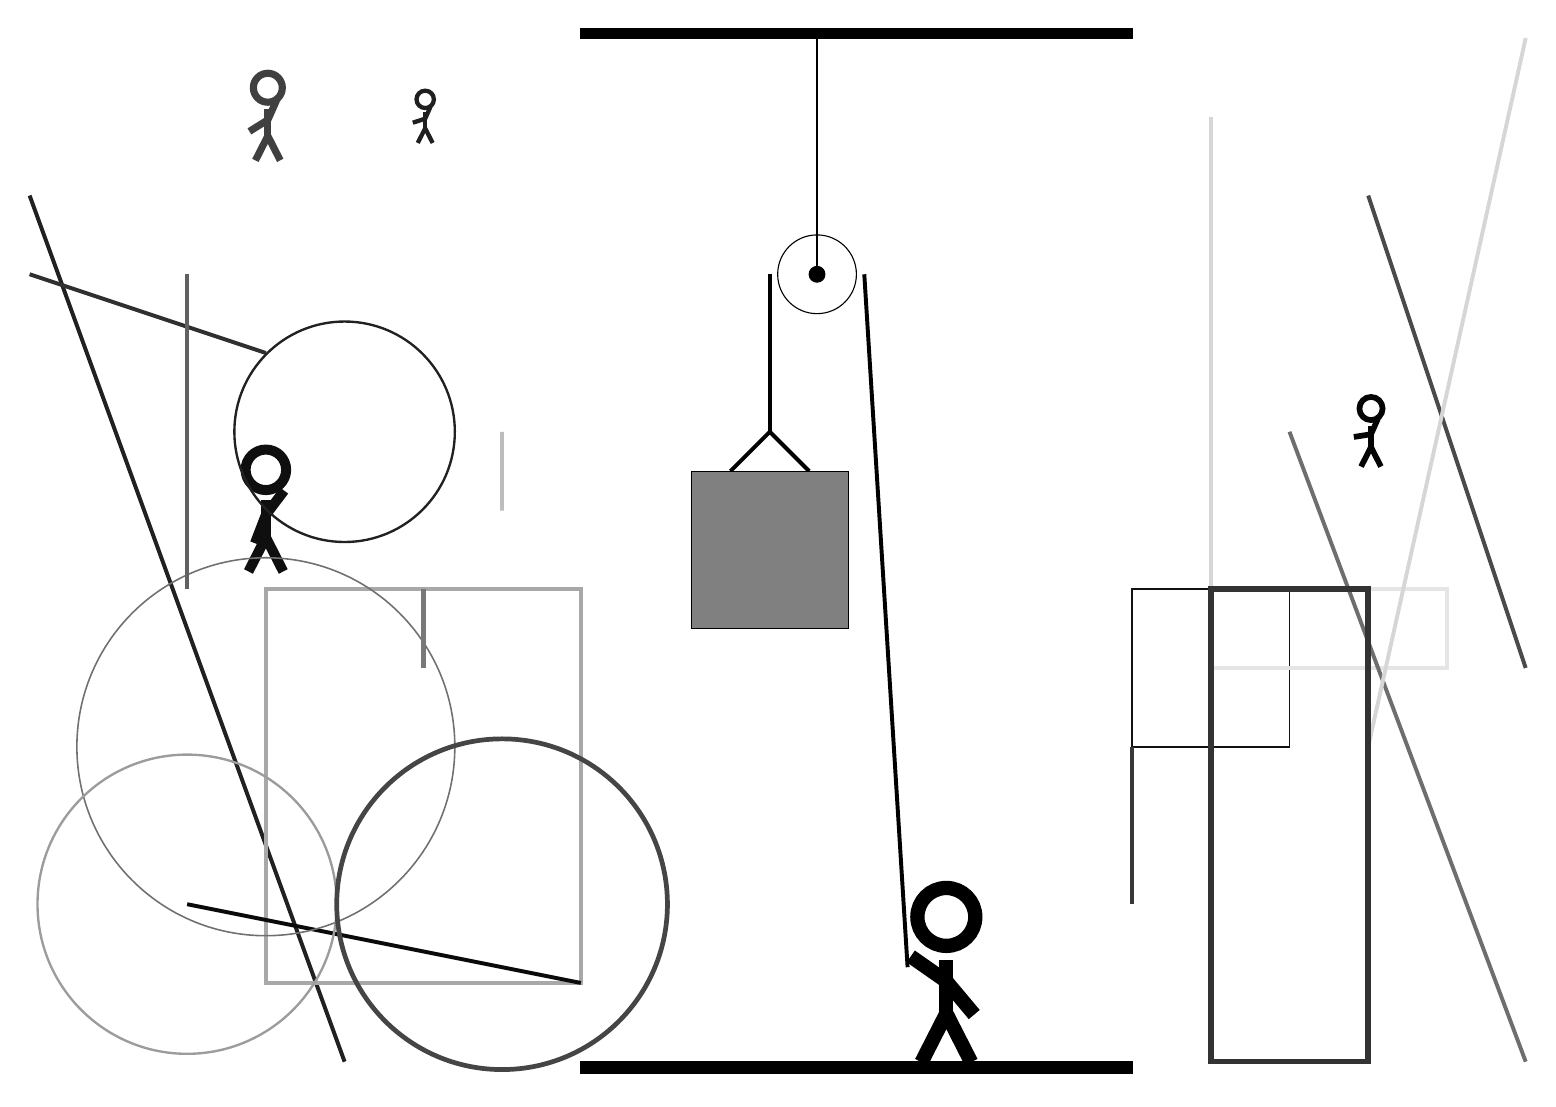
\begin{tikzpicture}
		%%%%% START %%%%%
		
		\draw[fill=black] (-2, 10) rectangle (5, 10.125);
		
		\draw (1, 7) circle (0.5);
		\draw[fill=black] (1, 7) circle (0.1);
		\draw (1, 10) -- (1, 7);
		
		\draw[line width=0.5mm] (-0.1, 4.5) -- (0.4, 5.0) -- (0.9, 4.5);
		\draw[fill=black!50] (-0.6, 4.5) rectangle (1.4, 2.5);
		
		\draw[line width=0.5mm] (0.4, 7) -- (0.4, 5.0);
		\centerarc[line width=0.5mm](1, 7)(0:180:0.6);
		\draw[line width=0.5mm](1.6, 7) -- (2.15, -1.8);
		
		\draw[line width=0.5mm, color=black!87](-5, -3) -- (-9, 8);
		
		\node[line width=0.4mm, color=black!75] at (-6, 9) {\Strichmaxerl[5][32][66]};
		\draw[line width=0.5mm, color=black!34] (-2, -2) rectangle (-6, 3);
		\node[line width=0.2mm, color=black!88] at (-4, 9) {\Strichmaxerl[3][18][66]};
		
		\draw[line width=0.5mm, color=black!71](10, 2) -- (8, 8);
		\draw[line width=0.2mm, color=black!93] (5, 1) rectangle (7, 3);
		\node[line width=0.6mm, color=black!94] at (-6, 4) {\Strichmaxerl[7][69][53]};
		\draw[line width=0.5mm, color=black!78](5, -1) -- (5, 1);
		\node[line width=0.3mm, color=black!98] at (8, 5) {\Strichmaxerl[4][9][66]};
		\draw[line width=0.5mm, color=black!16](6, -1) -- (6, 9);
		\draw [line width=0.2mm, color=black!77](9, 7) circle (0.0);
		\draw[line width=0.5mm, color=black!26] (-3, 5) rectangle (-3, 4);
		\draw[line width=0.5mm, color=black!96](-2, -2) -- (-7, -1);
		\draw[line width=0.5mm, color=black!10] (6, 2) rectangle (9, 3);
		\draw[line width=0.5mm, color=black!57](7, 5) -- (10, -3);
		\draw [line width=0.2mm, color=black!56](-6, 1) circle (2.4);
		
		\draw [line width=0.3mm, color=black!39](-7, -1) circle (1.9);
		
		\draw [line width=0.6mm, color=black!73](-3, -1) circle (2.1);
		\draw[line width=0.5mm, color=black!81](-6, 6) -- (-9, 7);
		\draw[line width=0.6mm, color=black!53] (-4, 2) rectangle (-4, 3);
		\draw[line width=0.5mm, color=black!16](8, 1) -- (10, 10);
		
		\draw [line width=0.3mm, color=black!87](-5, 5) circle (1.4);
		
		\draw[line width=0.5mm, color=black!62](-7, 7) -- (-7, 3);
		\draw[line width=0.7mm, color=black!80] (6, -3) rectangle (8, 3);
		
		\node at (2.6, -1.9) {\Strichmaxerl[10][-35][-50]};
		
		\draw[fill=black] (-2, -3) rectangle (5, -3.15);
		
		%%%%% END %%%%%
	\end{tikzpicture}
\end{document}